\documentclass[a4paper,12pt]{article} %style de document
\usepackage[utf8]{inputenc} %encodage des caractères
\usepackage[french]{babel} %paquet de langue français
\usepackage[T1]{fontenc} %encodage de la police
\usepackage[top=2cm,bottom=2cm,left=2cm,right=2cm]{geometry} %marges
\usepackage{graphicx} %affichage des images


\begin{document} %début du document



%----------------------------------
%page de garde
%----------------------------------

\begin{titlepage}

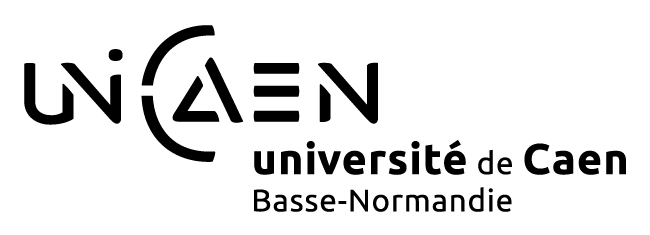
\includegraphics[scale=0.3]{images/unicaen.png}

\vspace{7cm}

\begin{center}

\begin{Huge}
Complément POO\\
Rapport du Devoir\\
\end{Huge}
\vspace{2cm}
\begin{large}
Beauchamp Aymeric 21301016\\
Chagneux Dimitri 21606807\\
Mori Baptiste 21602052\\
Leblond Valentin 21609038\\
\vspace{1cm}
L2-Info-groupe-4A
\end{large}

\end{center}
\end{titlepage}


%------------------------------
%sommaire
%------------------------------

\newpage

\tableofcontents{}

\newpage

%------------------------------
%contenu
%------------------------------


\section*{Introduction}
\addcontentsline{toc}{section}{Introduction}

L'objectif de ce projet de POO est de réaliser un taquin : un casse-tête consistant à déplacer des cases d'un plateau afin de les replacer dans l'ordre et ainsi reconstituer une image ou un motif donné.

\begin{figure}[!h]
\centering
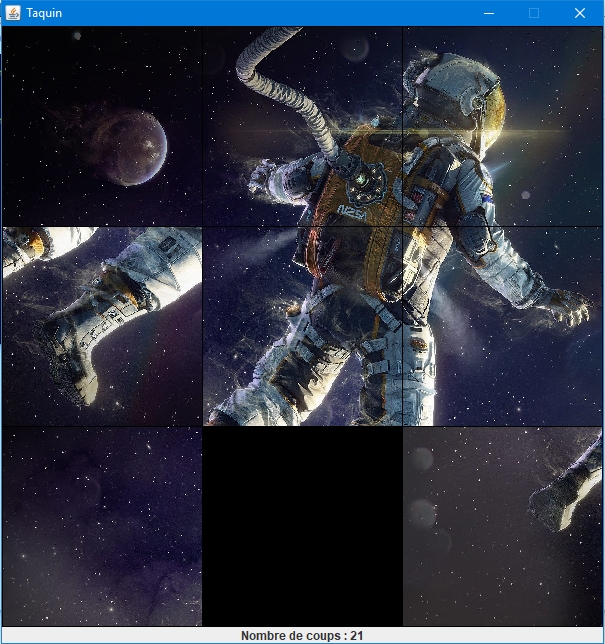
\includegraphics[scale=0.5]{images/Capture.PNG}
\caption{Jeu du Taquin}
\end{figure}

Nous avons séparé le projet en deux packages, le premier comportant le modèle du jeu utilisable en version console (le package \textbf{model}), et le deuxième, l'implémentation de l'interface graphique (le package \textbf{GUI}). Nous utilisons également un troisième dossier \textbf{ressources} où sont stockées les images utilisées par l'application.

\section{La conception du package model}

Le modèle de base du taquin est constitué d'une grille d'objets représentant les différentes cases. Les cases pleines ont des identifiants pour permettre de mettre en place la condition de victoire : on gagne si chaque identifiant est placé aux bonnes coordonnées.

\subsection{Organisation des classes}

Tout d'abord, nous avons représenté les cases par deux classes, \textit{\textbf{FullTile}} pour les cases pleines et \textit{\textbf{EmptyTile}} pour la zone vide qu'on déplacera. Ces classes possèdent des attributs en commun qui sont les coordonnées X et Y dans la grille ; c'est pourquoi nous avons conçu une classe abstraite \textit{Tile} qui possède ces coordonnées et dont héritent FullTile et EmptyTile.\\
La classe FullTile diffère de EmptyTile en ce qu'elle possède en plus un identifiant entier que l'on rend unique pour chaque instance utilisée.\\

Ensuite, nous avons une classe Board qui décrit l'état du jeu et le fait évoluer.

\begin{figure}[!h]
\centering
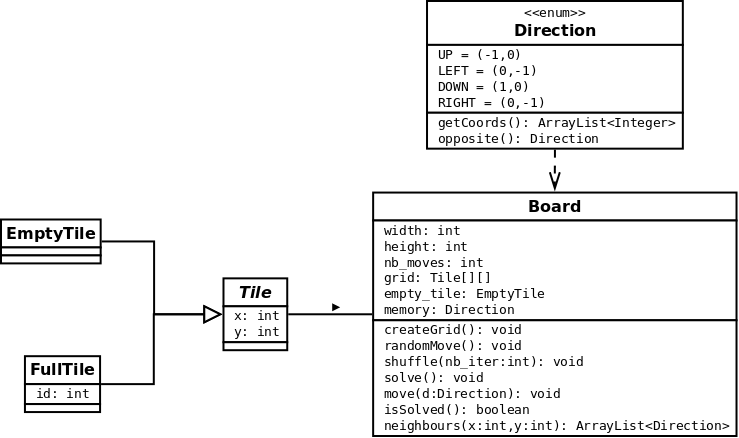
\includegraphics[scale=0.4]{images/model.png}
\caption{Diagramme de classe du package model}
\end{figure}

\newpage

\subsection{Fonctionnement du modèle}

Comme nous l'avons expliqué, l'initialisation et la mise à jour du modèle se font par le biais de la classe Board.\\

En premier lieu, nous avons une fonction \textbf{createGrid} qui permet d'initialiser une grille avec des FullTile et une EmptyTile et une fonction \textbf{toString} qui permet de l'afficher.\\
La grille ainsi créée est dans un état résolu où les identifiants des cases sont rangés dans l'ordre ci-dessous :

\begin{figure}[!h]
\centering
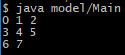
\includegraphics[scale=1]{images/Capture2.PNG}
\caption{Affiche d'une grille 3x3 initialisée}
\end{figure}

Puis, nous avons crée les déplacements de la case vide, nous avons d'abord commencer par créer une enum Direction avec quatre instances UP, DOWN, LEFT, RIGHT qui représentent une direction de déplacement. Nous utilisons cette enum dans la fonction \textbf{move} qui déplace la case vide dans la direction donnée en argument.\\

Pour mélanger le jeu, on choisit un mouvement aléatoire selon les mouvements possibles de la case vide puis on déplace la case vide jusqu'en bas à droite, à sa position initiale. On garde en mémoire le dernier coup effectué afin d'éviter des coups inutiles qui réduisent l'efficacité du mélange ; si l'on va vers le haut lors d'un coup, on interdit d'aller vers le bas au coup suivant.\\
Le mélange est effectué par la fonction \textbf{shuffle} qui prend en argument le nombre de coups à réaliser avant de considérer le mélange comme terminé. Dans la version finale, nous faisons 10 000 mélanges. Cela assure une bonne dispersion des cases pour un temps de calcul négligeable.\\
Comme la grille initiale est résolue, l'état obtenu par le mélange n'est pas bloquant puisqu'il existe une séquence de coups menant de cet état à la solution.\\

La récupération des coups jouables de la case vide est un voisinage de taille 4 de rayon 1 qui correspond aux quatre directions haut, bas, gauche, droite. La fonction \textbf{neighbours} donne selon une coordonnée dans la grille du jeu donne toutes les directions possibles.\\

Le modèle dispose aussi d'une fonction \textbf{solve} qui résout le puzzle. Nous avons utilisé une approche extrêmement simple consistant à jouer un coup aléatoire jusqu'à obtenir la configuration initiale de la grille.\\
Cette simplicité a un coût : le solveur peut réaliser jusqu'à 500 000 coups pour résoudre un simple puzzle 3x3, et devient très lent dès que l'on veut augmenter la taille.
Nous sommes conscients qu'il est possible de réaliser un solveur plus efficace, par exemple via l'utilisation de l'algorithme A*, mais nous avons préféré ne pas nous focaliser sur cet aspect du projet.\\

La classe principale permet de jouer au taquin en interface console. Le joueur peut déplacer la case vide avec Z,Q,S,D.

\section{Conception du package GUI}

L'interface graphique est composée de deux fenêtres, celle permettant de choisir l'image du jeu et la deuxième qui est le jeu en lui-même.

\subsection{Organisation des classes}

L'interface graphique est composée de vue \textbf{View}, du model \textbf{Board, Tile} et du contrôleur présent dans \textbf{Interface} (clics de souris et touches du clavier). La vue implémente \textbf{ModelListener} qui permet de l'actualiser lorsque un mouvement du model se fait. Le model (ici le \textbf{Board}) étend de \textbf{AbstractModeleEcoutable} qui permet d'ajouter ou supprimer des écouteurs mais aussi d'une méthode qui permet d'actualiser tous les écouteurs qu'on fera appelle lors de l'exécution de la fonction \textbf{move}. Les contrôleurs lancer le mouvement du model qui va lui actualiser la vue.

\begin{figure}[!h]
\centering
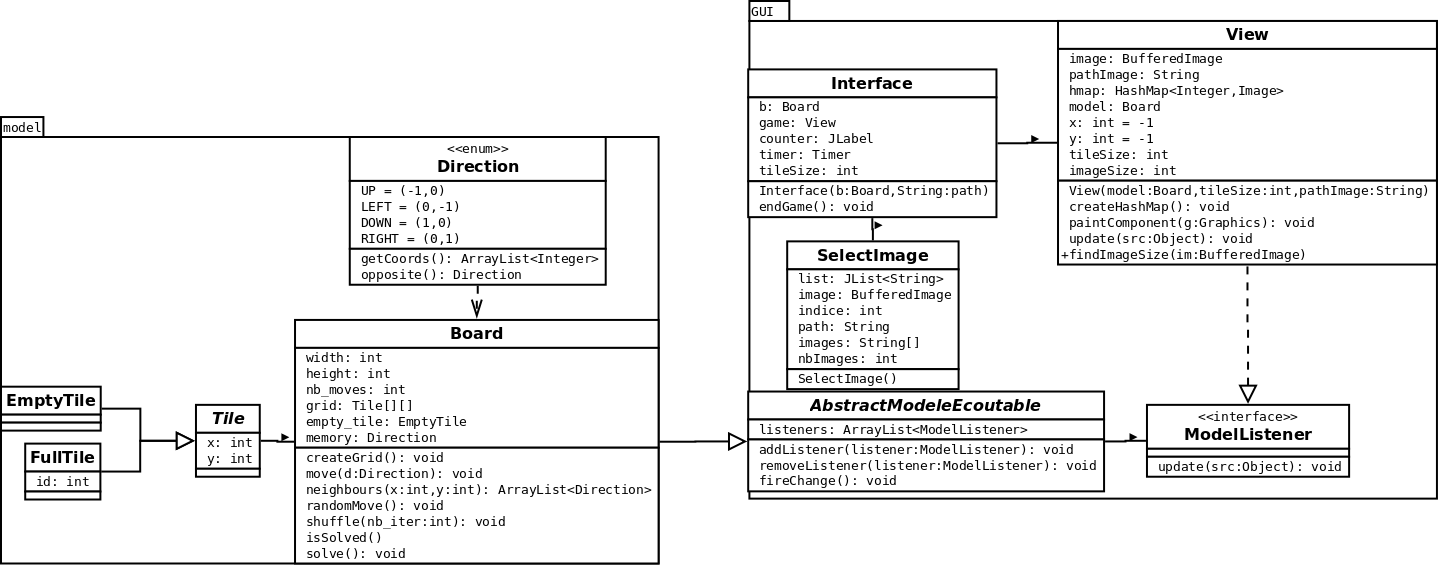
\includegraphics[scale=0.25]{images/mvc.png}
\caption{Diagramme de classe MVC}
\end{figure}
 

\subsection{Fonctionnement GUI}

D'abord, pour représenter l'état du jeu, la classe \textbf{View} permet à partir d'un chemin, d'une image et d'un Board découper l'image et lier pour chaque identifiant une partie de l'image qui lui correspond. La case vide ne possède pas d'identifiant et pourtant elle a une image qui est associé à son identifiant si elle en possédait un, c'est comme cela que quand le puzzle est résolut, on dessine toute l'image sans la case vide et on enlève aussi le quadrillage pour avoir l'image propre.

\begin{figure}[!h]
\centering
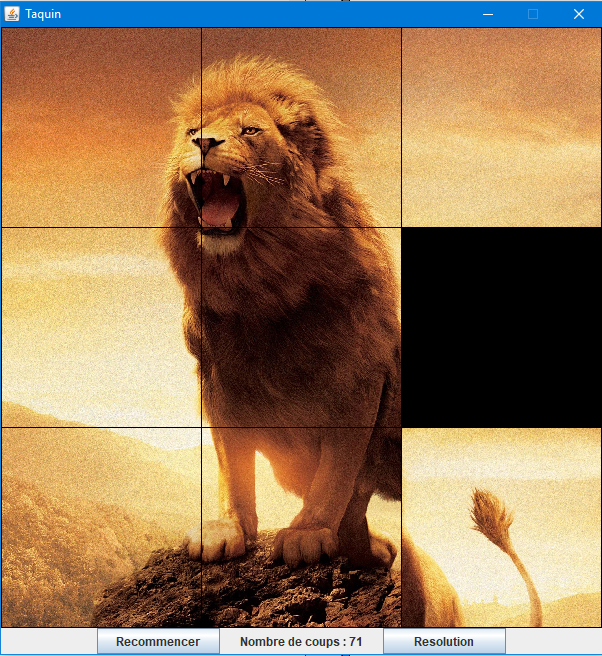
\includegraphics[scale=0.4]{images/Capture3.PNG}
\hspace{0.2cm}
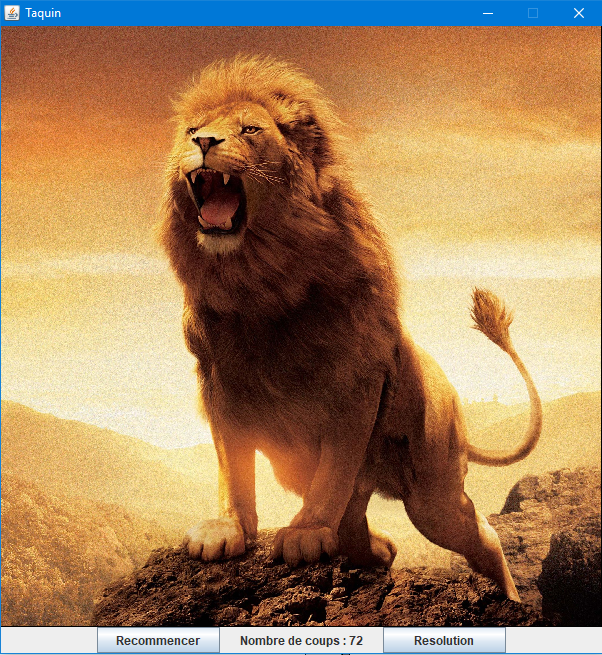
\includegraphics[scale=0.4]{images/Capture4.PNG}
\caption{Visuel de la résolution du Taquin}
\end{figure}

Pour choisir l'image qui est en fond, nous avons fait une autre interface qui va chercher tous les éléments qui sont dans le dossier \textbf{ressources} (qui sont que des images) et qui seront listé dans une liste (en utilisant JList, Vector et JScrollPane pour gérer une plus grande quantité d'image). On ajoute dans le vecteur que les noms des images sans l'extension et on créer la JList avec le Vector en argument. Ensuite on créer le JScrollPane et on ajoute la JList. Pour ajouter le tout, on ajoute le JScrollPane de la même manière qu'un JPanel avec un \textbf{add} dans la frame. Quand on sélectionne une image dans la liste, elle s'affiche sur la droite de la liste. Enfin, une fois l'image voulu sélectionné, en appuyant sur le bouton \textbf{Jouer} on lance l'interface du jeu avec l'image choisi en fond. Toutes les images sont possible d'ajouter pour le format et la taille mais si l'image est petite, elle sera étendu et le visuel sera pixelisé.

\begin{figure}[!h]
\centering
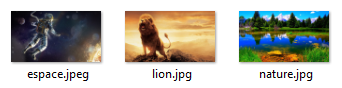
\includegraphics[scale=0.8]{images/Capture5.PNG}
\caption{Images dans le dossier \textbf{ressources}}
\end{figure}

\begin{figure}[!h]
\centering
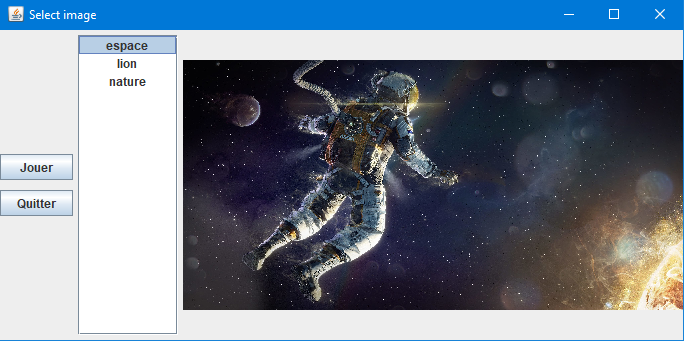
\includegraphics[scale=0.6]{images/Capture6.PNG}
\newpage
\vspace{0.1cm}
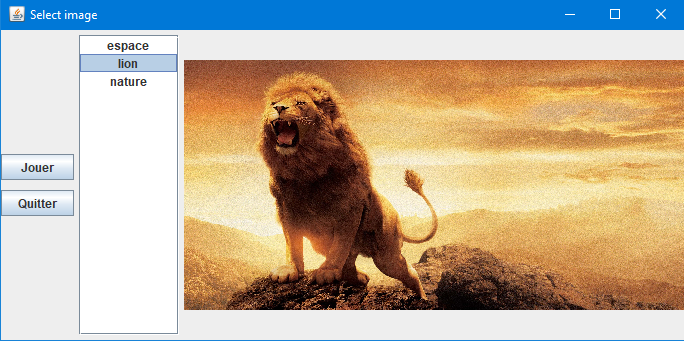
\includegraphics[scale=0.6]{images/Capture7.PNG}
\caption{Interface de séléction d'image}
\end{figure}

\newpage

Les déplacements sont fait soit avec le clic de la souris ou soit avec les flèches directionnelles du clavier.\\
Pour le déplacement de la souris, on récupère la position du clic et on le divise par la taille que les cases ont et enfin on prend la partie entière ce qui nous donne les coordonnées en cases du clic de souris. Il nous reste maintenant à tester si le clic de la souris correspond à une énums, on va soustraire les coordonnées de la case cliquée avec la case vide ce qui nous donne le vecteur de déplacement et si ce vecteur correspond à une des énums des positions jouable de la case vide on effectue le mouvement sinon on fait rien.\\
Pour le déplacement au clavier, c'est plus simple, on teste qu'elle touche est pressée et si c'est la touche du haut on lance la fonction \textbf{move} du Board (qui test si la case de destination est dans la grille), de même pour les autres directions.\\

Un bouton \textbf{recommencer} et \textbf{resolution} sont présent en bas de l'interface de jeu qui permettent respectivement de recommencer le jeu et de le résoudre. Pour recommencer le jeu, on a juste à mélanger le jeu.

\section*{Conclusion}
\addcontentsline{toc}{section}{Conclusion}

L'objectif du projet a été atteint, nous avons réalisé le jeu du Taquin jouable en console et une version jouable en interface graphique.\\

Nous aurions pu améliorer ce projet par exemple en proposant au joueur les dimensions de la grille de jeu que nous avons mis par défaut en 3x3 mais nous avons fait en sorte que la grille et l'interface soient adaptatif aux dimension de la grille.

\newpage

\begin{figure}[!h]
\centering
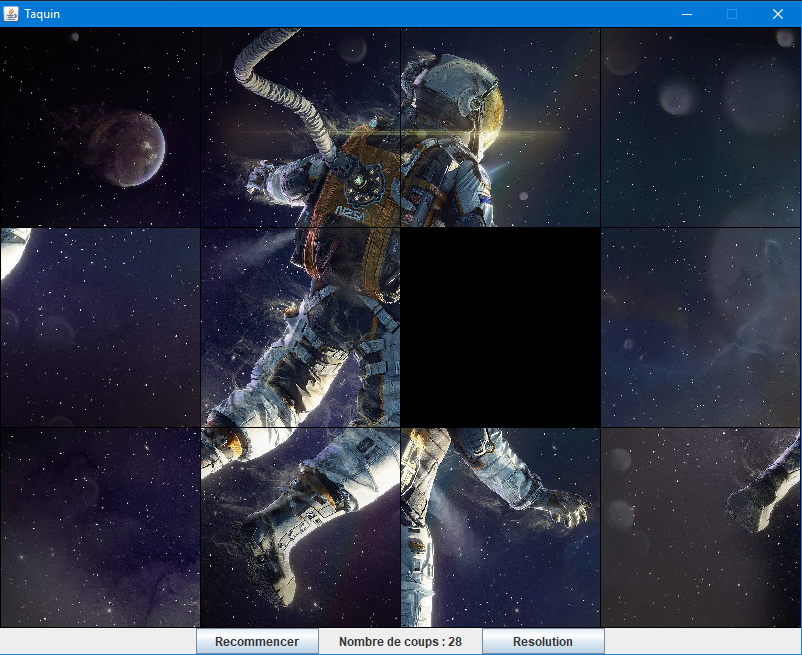
\includegraphics[scale=0.6]{images/Capture8.PNG}
\caption{Interface graphique avec une dimension 4x3}
\end{figure}

\end{document}
